\documentclass[10pt,twocolumn,letterpaper]{article}

\usepackage{todonotes}
\usepackage{iccp}
\usepackage{times}
\usepackage{amsmath}
\usepackage{amssymb}
\usepackage{url}
\usepackage{graphicx}
\usepackage[pdftex,pdfpagelabels,bookmarks,hyperindex,hyperfigures]{hyperref}

\iccpfinalcopy

\def\httilde{\mbox{\tt\raisebox{-.5ex}{\symbol{126}}}}

% Pages are numbered in submission mode, and unnumbered in camera-ready
\ificcpfinal\pagestyle{empty}\fi
\begin{document}

%%%%%%%%% TITLE
\title{Clipping-based Virtual Environment}

\author{Andrew Soohwan Lee\\
Stanford University\\
{\small\url{https://andrewlee.design/}}
}

\maketitle
\thispagestyle{empty}

%%%%%%%%% ABSTRACT
\begin{abstract}
This paper explains the creation of \textnormal{Cracking the Egg}, a virtual reality (VR) scene which explores the concept of using the near-clipping plane of the user camera to clip into objects and see inside them. It discusses related works to this concept and the game's features, and also outlines potential methods of expanding upon the initial scene.\\
\end{abstract}

%%%%%%%%% BODY TEXT
\section{Introduction} \label{introduction}

With the introduction of head-mounted displays (HMD's) as mass-market consumer products, independent content creators and programmers have gained the ability to create for a new platform afforded by virtual and augmented reality.

This paper follows the creation, motivations behind, and effects of creating a virtual environment in which a user is proactively told to clip into 3D objects (using positional tracking to physically enter normally-solid forms).

\subsection{The Scene}

This scene, called \textit{Cracking the Egg}, is modeled around the premise of being a "computer hacker" in the future, using a program called an \textit{Egg} to crack a passcode. A simple environment is created simulating this world where the player must clip into the metaphorical "egg" and look around miniature scenes with hidden objects (i.e., move the viewer's camera through an object, and "clip" into it by not rendering anything before the near-clipping plane). A computer panel is stationed next to the egg, which is used by the player to control which scene is displayed.

The overarching theme of the game is that the miniature objects represent "keys" to the passcode, in the same vein of cryptographic keys used today. However, they are all represented in physical representations (such as a cow or a car) hidden away in virtual mini-scenes inside of the program.

Ultimately, by manipulating and repositioning oneself around the scene, the player is able to "crack the egg" and uncover the passcode by finding each of these hidden objects.

\subsection{Motivation}

This VR scene was motivated primarily by an interest to study and implement a virtual scene in the game engine Unity. I was provided an Oculus Rift CV1 for my use, which includes an HMD, a positional tracking camera, and a remote with a directional-pad.

It was the option to use positional tracking that motivated me to explore the ability to manipulate and work with an environment by physically moving around it.

\subsection{Objectives}

The objectives this project began with are as follows:

\begin{enumerate}
  \item Create an interactive VR game with orientation and positional tracking using an Oculus Rift CV1
  \item Design and create 3D models that join together into a larger scene using Blender (with a "low-poly" style to save time)
  \item The user can manipulate the scene by walking around it, moving closer to it, and "looking" at parts of the object (i.e., clipping the camera through the object's walls)
  \item Create an immersive atmosphere using sound, lighting effects, and minimal animation
\end{enumerate}

%-------------------------------------------------------------------------

\section{Related Work}

\subsection{Existing VR Media}

Some recent VR media and tools have demonstrated or utilized the ability to use the near-clipping plane as a tool for storytelling, or a better understanding of the inner-workings of an object.

\begin{figure}[t]
\begin{center}
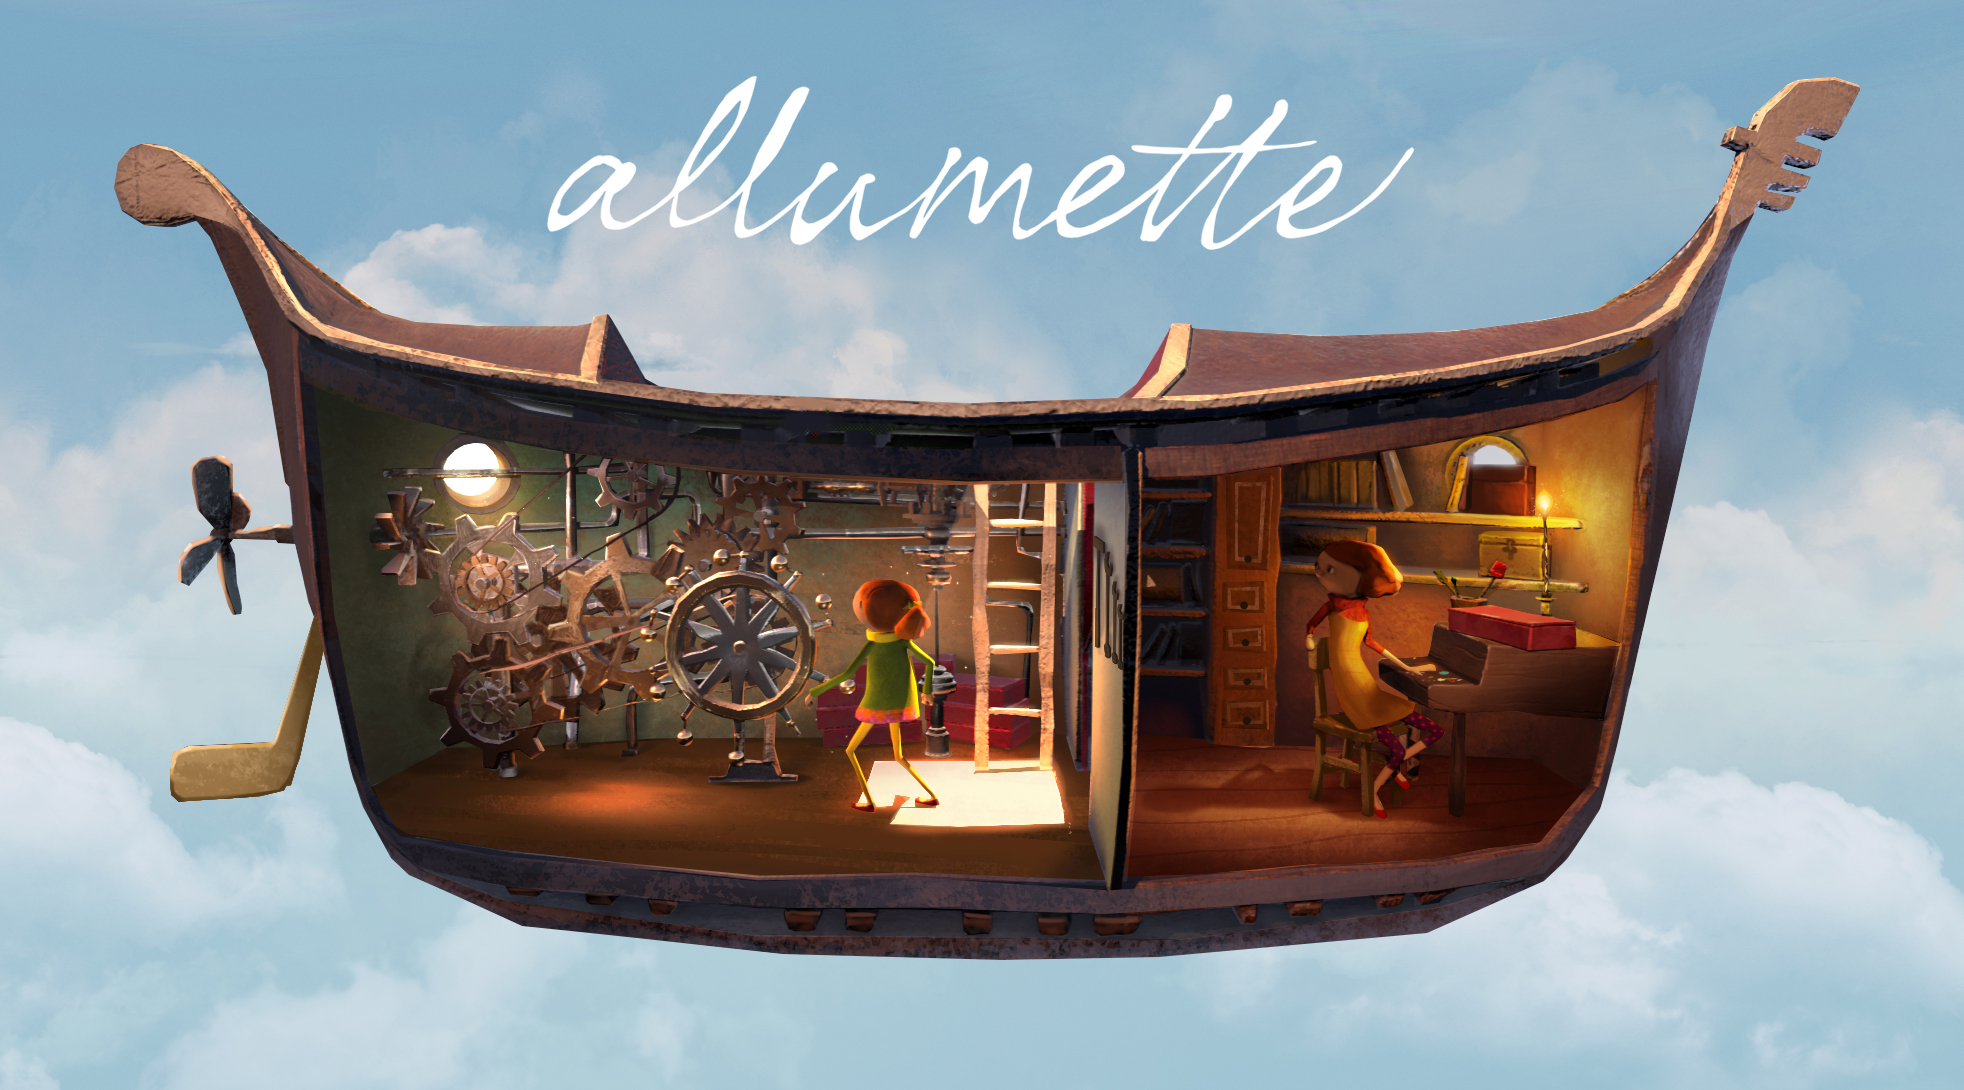
\includegraphics[width=1.0\linewidth]{images/allumette.jpg}
%\fbox{\rule{0pt}{2in}\rule{0.9\linewidth}{0pt} }
\end{center}
   \caption{\textit{Allumette}.  The viewer is able to peek into a flying ship by physically positioning its wall outside the bounds of the near-clipping plane. }
\label{fig:long}
\label{fig:onecol}
\end{figure}

\textit{Allumette} is a VR movie produced by Penrose Studios, which explores the life of an orphaned child in a 19th century fantasy world. In it, the viewer is given a god-like perspective over the story's floating city, and sees its characters and props as miniature figures the viewer can walk around and inspect ~\cite{Allumette}. In one scene, the viewer is able to clip into a flying ship on fire, and see the struggle of the main character's mother attempting to fly her ship away before it explodes and destroys the city. By peeking into the ship (clipping into it), the viewer is given a first-hand perspective within the context of the larger city scene.

It is important to note that the viewer is given complete control over their position in the scene, so they could otherwise ignore this entire moment. Therefore, the viewer is given a choice of control over how invested they are into the scene. This ability to clip into the ship may be unknown to a user who is not familiar with VR or their ability to do so.\\

\begin{figure}[t]
\begin{center}
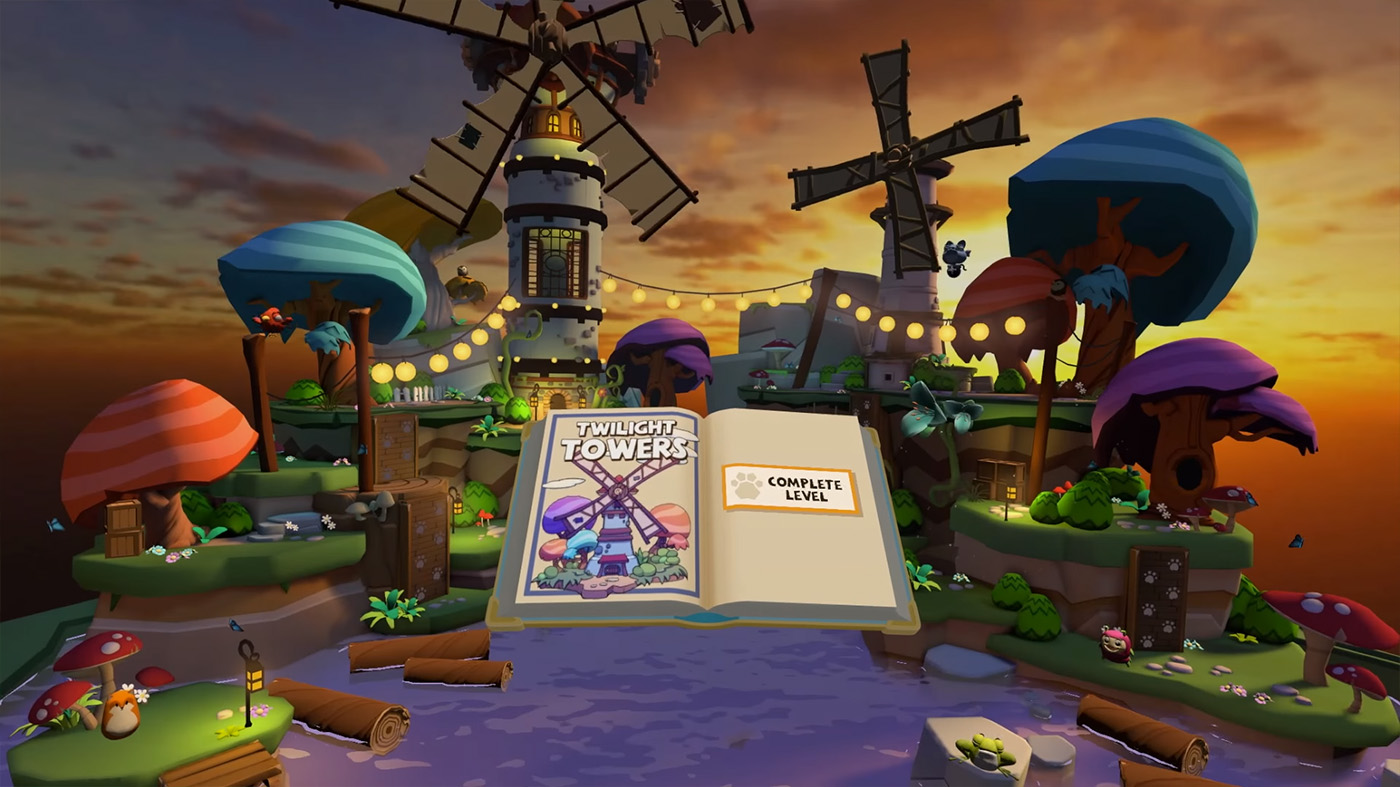
\includegraphics[width=1.0\linewidth]{images/luckystale.jpg}
\end{center}
   \caption{\textit{Lucky's Tale}.  The level select screen of this game allows the user to walk around and peek closer at a miniature world. }
\label{fig:long}
\label{fig:onecol}
\end{figure}

\textit{Lucky's Tale} is another example of creating a miniature world that the player can step closer to and clip into. The game features a cartoon world with standard 3D platforming gameplay ~\cite{LuckysTale}. However, what makes this game unique is how it gives the player a god-like perspective similar to \textit{Allumette}, where the player follows a miniature fox as it goes through the virtual world. In the level-select screen, the player is able to position their head and body around a storybook and look closer at the lives of the island's inhabitants.

The user is also able to clip into miniature aspects of these scenes, like to look into the interior of a windmill in the level select screen. Again, this provides a stronger sense of immersion by giving the player control over their view.\\

\begin{figure}[t]
\begin{center}
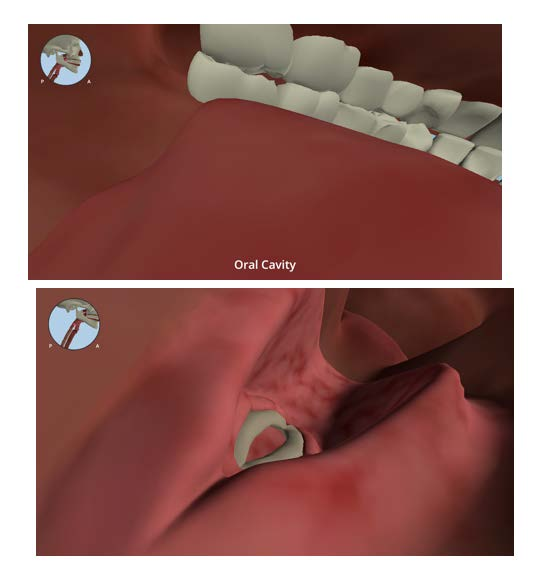
\includegraphics[width=1.0\linewidth]{images/anatomyou.jpg}
\end{center}
   \caption{\textit{Anatomyou}.  Users are given the ability to look into and explore human organs and body parts. }
\label{fig:long}
\label{fig:onecol}
\end{figure}

\textit{Anatomyou} is a medical anatomy simulator that teaches by showing viewers 3D models of human body parts and organs. The program demonstrates the ability to clip into objects in order to see their inner-workings, such as for an example provided by the program which displays a giant human heart with sample blood cells moving around its chambers. A user can walk around the heart, or even position themselves inside of it to gain a better understanding of how the entire construction behaves. Jaunes \etal discuss how "[t]hrough binocular vision we are able to appreciate different distances and volumes of our surrounding environment" ~\cite{Juanes:2016:IVA:3012430.3012559}.

\subsection{User Interface Design}

Prior works have explored the interplay in User Interface (UI) design between 2D and 3D interfaces. Particularly in VR, it is crucial to provide reactive tools that the user can intuitively understand, given not only past contexts of computer interfaces, but also physical tools as well. The relatively jarring and novel introduction to VR for new users can also be a source of confusion that

Kang discusses the importance of balancing the usage of 2D and 3D interfaces when creating virtual interactions ~\cite{7892351}. They discuss past research demonstrating how 3D objects can be used to quickly understand the purpose of an application, but not how to use it.

Doug, Ernst \etal explore the differences between 2D and 3D interfaces, calling attention to how 2D interactions can often be more efficient than 3D ones. In fact, they conclude that a "magic" interface, one which ignores physical constraints or abilities, should be preferred over mimicking physical reality, unless doing so is important to the application. They attribute this to the necessity to better structure the extra dimension of interaction, which is both unfamiliar to users and more cumbersome in terms of the movement required and interpreting intent ~\cite{442977420010201}.

\subsection{Visual Discomfort}

It is generally established that discomfort and simulator sickness when using HMD's is in-part caused by distances in VR being perceived at an incorrect distance due to the physical nature of the digital display being static. Peer discusses how \textit{distance compression}, the frequent underestimation of distance by users, has potential solutions through perceptual calibration and adaptation ~\cite{7892353}.

Prior work on visual discomfort when using HMD's has demonstrated how visual strain is more severe due to long-term focus without accommodation, rather than purely the vergence-accommodation conflict. ~\cite{7892270}.

%-------------------------------------------------------------------------

\section{Methods}

\subsection{Hardware}

The hardware used to create \textit{Cracking the Egg} included an NVIDIA GTX 970 Graphics Card, enclosed in an external GPU setup, powering an Oculus Rift. The Rift included an Oculus Remote and a positional tracking camera. All three of these components were directly used in the implementation of the scene.

One limitation of the hardware was only having a single positional tracking camera, which made movement and tracking when facing away from the camera unresponsive and jittery.

\subsection{Creation of the Scene}

The virtual environment itself was created in the Unity game engine, using models both created in Blender 3D and downloaded from the Unity Asset Store. All design considerations were based on a "low-poly" style, which allowed for rapid creation and iteration on objects without worrying about photorealism.

Oculus, the creator of the Oculus Rift, provides a Unity-based software development kit (SDK) called OVR for developers to utilize, which provides general integration with the hardware, along with specific tools and menus that facilitate development. Specific scripts used included those for spatial audio, gaze-based pointing, and VR Ray-casting.

Over the course of two weeks, the virtual scene was developed with a specific plan of learning to use the game engine, and piece-by-piece integrating specially-created models from Blender. The concept for the overarching story behind the scene was developed in reference to a television show, \textit{Black Mirror}, one episode of which describes the usage of a metaphorical egg that copies a human's personality. The theme of being in an incubator working as a computer hacker was developed in brief bursts of brainstorming ways to add a story to the scene.

The project was completed in an open-source git repository, which is linked in section \ref{opensource} of this paper.

\subsection{Features Implemented}

In total, five miniature environments were developed along with an exterior one that surrounds the egg. Each environment displays a different world, such as a desert landscape or a mountain shrine, and also emits ambient spatial audio that is heard only when the user is clipped into the egg.\\

One important feature implemented with help from the OVR Unity package is gaze-based interactions. The essence of this interaction method is that the user is given a "gaze-pointer" which, in the case of \textit{Cracking the Egg}, is a blue glowing circle that acts like a mouse-cursor. The cursor is aligned to the center of the user's view in the scene, and can be used to select menu options or "click" on objects with the Remote hardware.

This is implemented in the engine by using a raycast from the user's camera and detecting any collisions with the scene.\\

Another feature that was added were two virtual panels next to the egg that the player could use to manipulate the world. On each panel were different user interface elements that directly caused actions such as initializing the egg, or causing the egg to change its inner-scene. These panels were implemented using Unity's UI system incorporating the OVRRaycasting script from Oculus. The user can interact with these panels using gaze-based pointing, and they emit audio and visual effects as feedback to the user.


%-------------------------------------------------------------------------

\section{Evaluation}

\begin{figure}[t]
\begin{center}
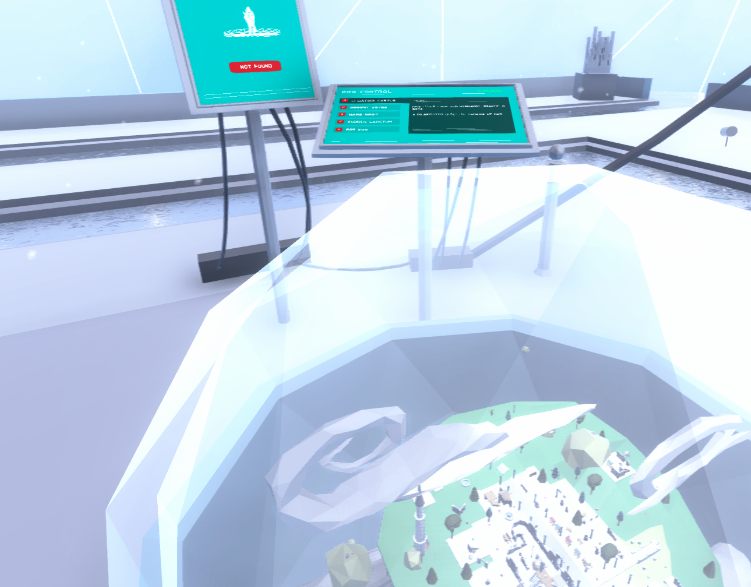
\includegraphics[width=1.0\linewidth]{images/crackingtheegg.png}
\end{center}
   \caption{\textit{Cracking the Egg}.  The player is put into a virtual world with the egg (the translucent icosphere), which they are able to clip into. }
\label{fig:long}
\label{fig:onecol}
\end{figure}

\subsection{Completion of Objectives}

Each objective was completed satisfactorily, and in fact, the project took on a much larger scale than expected. At first, the concept was just to be able to walk around a virtual scene and clip into objects. However, as it went on, additional features were added, such as the computer screen to change the environment inside the egg, and the addition of an objective to win the game (finding all the hidden objects). These extra components help to develop how immersive the environment feels for a user, allowing for more control and a sense of efficacy.

\subsection{User Testing}

\textit{Note: these are personal observations, and are not empirical.}\\

The project was demonstrated during a demo-day at Stanford University, and approximately three dozen people experienced the scene. Generally, players were able to understand the scene given some context, and about 1/4th of them were able to find all five hidden objects (some with great ease). Participants' ages ranged from seven years old to about 60, and all were able to have a general understanding of how the virtual environment worked.

\subsection{Areas of Improvement}

One primary area of improvement found from user-testing was a need for better positional tracking. By only using a single Oculus Rift tracking camera (due to hardware limitations), users would often turn around to look at the egg in the scene, and see jarring jumps in vision or a lack of responsiveness from the scene. This was because the user's back would prevent a visual line of sight from the Rift camera to the markers on the back of the HMD. While this is more of a hardware constraint, the scene itself could be rearranged to prevent the user from needing to turn around so often.

Another area of improvement is the need to better introduce the virtual environment to the user, particularly for those who are new to VR. In terms of gaze-based pointing, it was very unintuitive for new users to understand at first, which led to a greater barrier to entry.

%-------------------------------------------------------------------------

\section{Discussion}

\subsection{Developing the Interface}

UI design served as an essential part of creating the virtual scene. While the project's initial intentions were to demonstrate the effect of clipping into objects, it became apparent that this action represented an entirely new interaction in-itself: being able to physically move within an interface. It brought to light the interplay between 2D and 3D interfaces, as discussed by Kang, where certain interactions are better suited in 2D, and others in 3D ~\cite{7892351}.

Given my personal background in 2D user interface design, particularly for websites, it was easy to feel tempted to resort to familiar UI patterns and techniques. The end result of \textit{Cracking the Egg} demonstrates this, given how the two panels are flat interfaces that the user can interact with. They are familiar and modeled off of existing design concepts like model boxes and tab-based panels.

While these ideas work in terms of a user interface, the medium of VR offers much more than digital representations of already existing concepts. These panels could have been pushed further — or, in fact, perhaps they were not needed at all. Their interfaces and physical presence provided a familiar sense of working with computers, yes, but they also served as a limiting way to interact with the 3D scene. For example, the user could have been taught a hand gesture or swiping action to "swipe through" the different environments, rather than having to turn back and forth between the panels and the egg.

\subsection{Understanding Gaze-based Pointing}

\begin{figure}[t]
\begin{center}
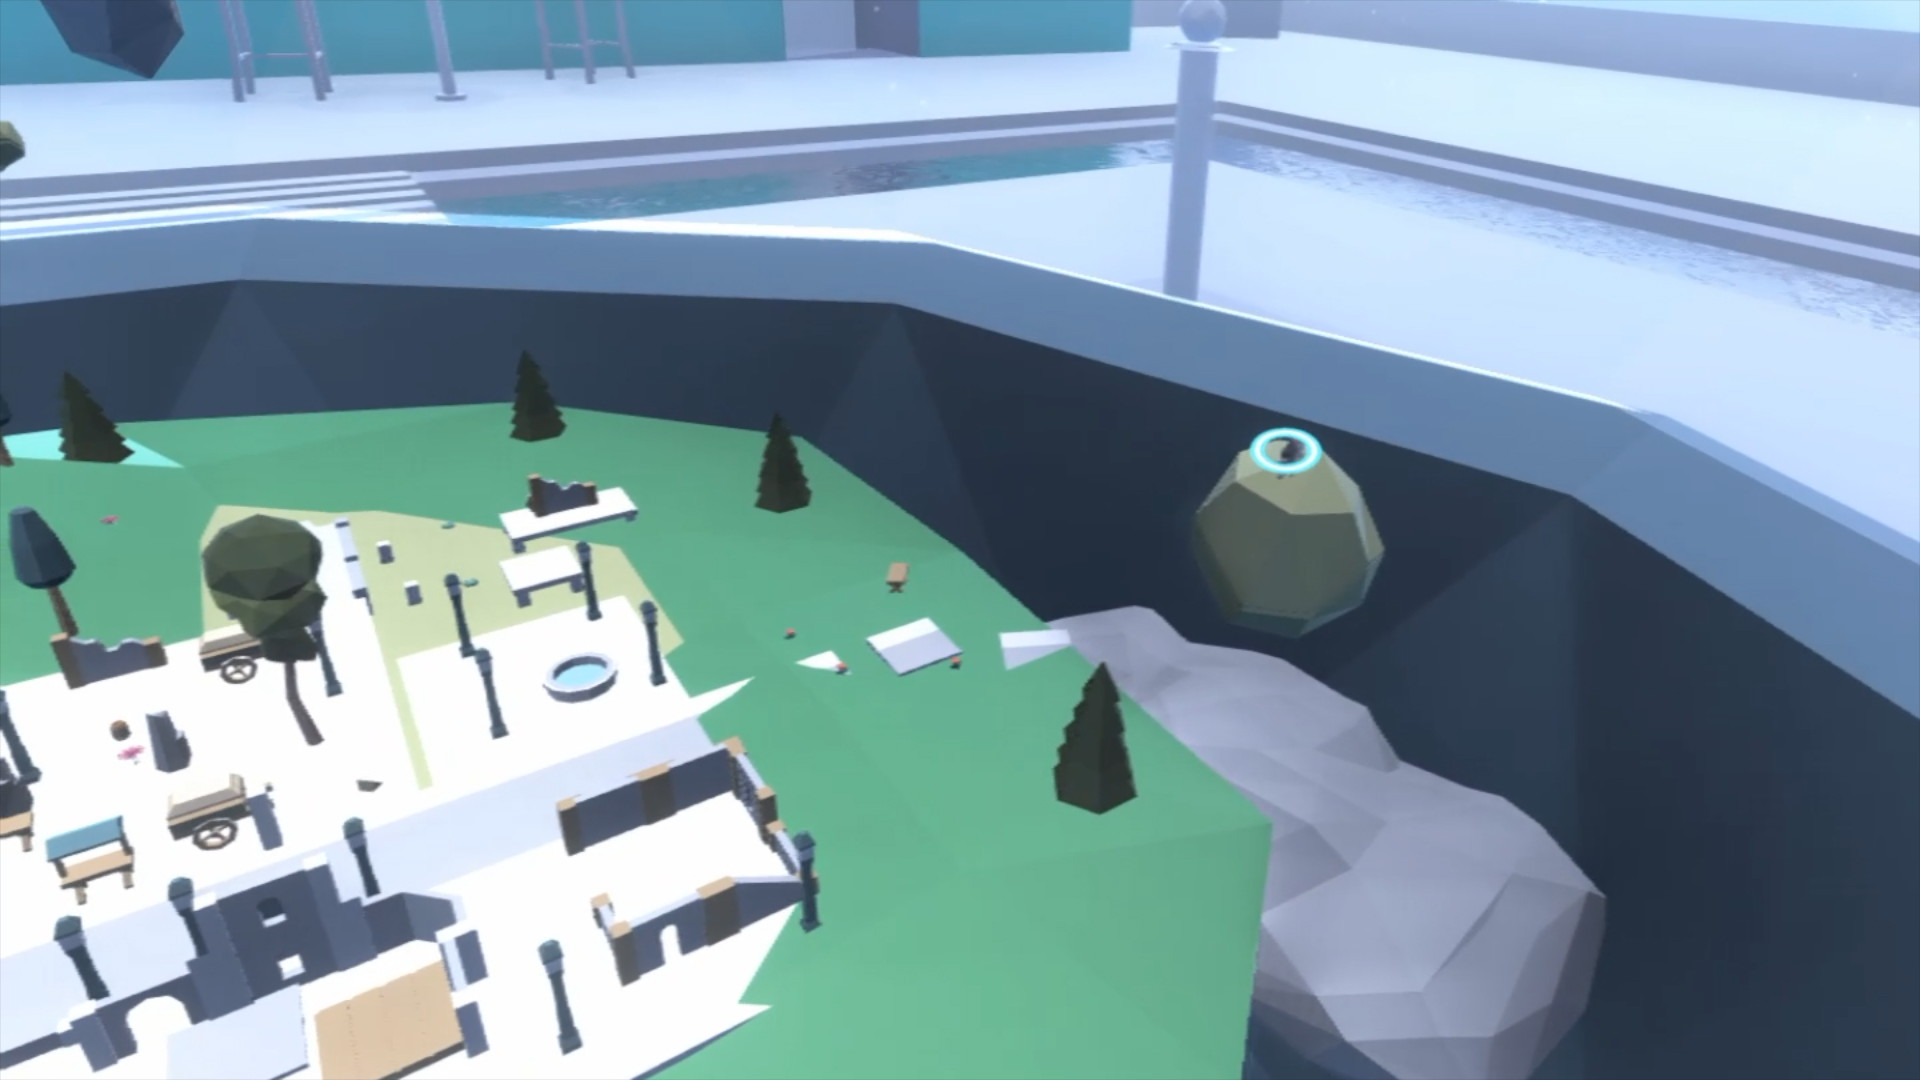
\includegraphics[width=1.0\linewidth]{images/gazepointing.jpg}
\end{center}
   \caption{ Gaze-based pointing was particularly difficult to understand for users who have not had much experience with VR. This interaction model is shown by the blue circle hovering over the rock on the right. }
\label{fig:long}
\label{fig:onecol}
\end{figure}

A common observation during testing with users was difficulty adapting to the gaze-based pointing if they were unfamiliar with VR.

One study by Atienza \etal discusses how its writers can "foresee the integration of many more gaze-based actions in future applications" due to its ability to be more reliable than other potential input interactions at the present moment \cite{7519387}. While today in 2017, Oculus and the HTC Vive have both introduced hand-tracking controllers to the market, both of these require much more physical movement and can be unreliably tracked for interface interactions. The study also brings to attention how  gaze-based pointing can be less intuitive, which is exactly what was demonstrated by users who were new to VR who tried the virtual scene. They had difficulty understanding how to interact with the world, and made assumptions that the Oculus Remote was tracked in space and would act like a mouse cursor.

This difficulty with gaze-based pointing is interesting in the context of the now rapidly-developing VR headset industry. The development of new hardware has created the ability to test out new interaction methods, but it is still unclear which is the most ideal for specific situations. For example, the home launcher app for the Oculus Rift uses gaze-based interactions to navigate the user around their game library and a virtual shop. However, this can feel cumbersome because the user needs to directly look at every object or interface element they wish to use, which can lead to head- or neck-strain overtime. Clearly, time will tell which methods of input are the most comfortable and user-friendly, but there are still barriers in place due to the technology's novelty and its rapidly changing pace.

\subsection{Eye Strain and Simulator Sickness}

\subsection{Hesitation to Embrace Virtual Media}

Another observation of users testing the VR scene was a tendency to resist fully committing to the environment, potentially due to self-consciousness, a lack of trust in the medium, or fear of hurting oneself. When demoing in the lab, an essential part of the scene asked users to essentially kneel down in front of them and walk around in a particularly crowded area. The first person to try out \textit{Cracking the Egg} was a young boy, who appeared to have no trouble at all walking around and experiencing the scene. However, as older participants (20 years and older) tried it out, they were more likely to question whether or not they should lean in or actually perceive the egg as a physical object on the ground.

This tendency appeared to be influenced by a number of factors. For one, the participants may have been more likely to feel embarrassed leaning down and acting in the scene, especially due to the large number of people around them (in reality). Another observed reason was that users who had not experienced VR before were more likely to hesitate walking around the space because it was a completely unfamiliar and potentially threatening environment. One last explanation could be that older users were more risk-adverse and less willing to enact quick movements or completely move their entire bodies.

\subsection{Conclusion}

\textit{Cracking the Egg} demonstrates the concept of making a virtual environment that actively encourages users to clip into the walls of otherwise physical objects. It integrates a variety of current knowledge and tools for the platform, while also serving as ways to look at the limitations of what exists in terms of visual discomfort and user interface design.

%-------------------------------------------------------------------------

\section{Miscellaneous}

\subsection{Open Source} \label{opensource}

The project is open source at \url{https://github.com/andrewsoohwanlee/Cracking-the-Egg} under an MIT License.

All assets used to create the scene are also listed in the Readme.md file in this repository.

\subsection{Acknowledgements}

Special thank you to Gordon Wetzstein, Robert Kondrad, Hayato Ikoma, and Keenan Molner for teaching \textit{EE 267: Virtual Reality} (Spring, 2017) at Stanford University.

{\small
\bibliographystyle{ieee}
\bibliography{egbib}
}

\end{document}
